\chapter{Laplace Transform}
\section{Definition}
The Laplace Transform is defined as 
\[ \laplaceMath{f(t)} = \int_{0}^{\infty}e^{-st}f(t) dt\] 
This transform is also one-to-one. This is useful when using the Laplace Transform to solve differential equations. 
\begin{example}
	Find \laplace{1}
	\begin{align}
		\laplaceMathComplete{1} \\
		= -\dfrac{1}{s}\left[e^{-st}\right]^\infty_0 \\
		= -\dfrac{1}{s} \left[ \dfrac{1}{e^{ \infty}} - \dfrac{1}{e^0} \right] \\
		\laplaceMath{1} = \dfrac{1}{s}
	\end{align}
	There are Laplace Transform Tables available that show the value of the transform for some obvious functions. 
	
\end{example}
\section{Solution to Initial Value Problems}
Consider the Laplace transform of the derivative of a function $ \laplaceMath{f'(t)} $ we get an interesting solution when we do the transform 
\begin{align}
\laplaceMathComplete{f'(t)} 
\intertext{Using integration by parts we find}
u = e^{-st} && du = -se^{-st} dt\\
dv = f'dt && v = f(t) \\
= \left[ e^{-st}f(t) \right]^\infty_0 - \int^\infty_0 -sf(t)e^{-st}dt
\laplaceMath{f'(t)} = -f(0) + s \laplaceMath{f(t)}
\end{align} 
We can find $ f'' $ as such and also find a similar pattern appear. 
\section{Using Laplace Transform to Solve Differential Equations}
The property that allows us to use Laplace Transform is that it is one-to-one. As in each function has a unique transform, and that transform can only have that one function that gives that result. 
\begin{example}
	Find the solution of the differential equation 
	\begin{align}
		y'' + y = \sin 2t \\ 
		\intertext{Satisfying the initial conditions}
		y(0) = 2, \indent y'(0) = 1
		\intertext{We begin by applying the transform to both sides of the equation}
		\laplaceMath{y'' + y} = \laplaceMath{y''} + \laplaceMath{y} = \laplaceMath{\sin 2t} \\
		\intertext{Expanding and plugging in the intial conditions we get}
		s^2 \laplaceMath{y} - 1 - 2s + \laplaceMath{y} = \dfrac{2}{s^2 + 4} \\
		\laplaceMath{y} [s^2 + 1] = \dfrac{2}{s^2 + 4} +1 + 2s \\
		= \dfrac{2s^3 + s^2 + 8s + 6}{s^2 + 4} \\
		\laplaceMath{y} = \dfrac{2s^3 + s^2 + 8s + 6}{(s^2 + 4)(s^2 + 1)}
		\intertext{Solving it you get}
		\laplaceMath{y} = \dfrac{2s}{s^2 +1} + \dfrac{5/3}{s^2 + 1} - \dfrac{2/3}{s^2 + 4} \\
		\intertext{Taking the inverse Laplace Transform}
		y(t) = 2 \cos t + \dfrac{5}{3} \sin t - \dfrac{2}{3} \sin 2t
	\end{align} 
\end{example}
\section{Mid-Section Assessment}

	\begin{q}
		Define the Laplace Transform for a function $ f(t) $
	\end{q}
	\begin{q}
		Find \laplace{1}
	\end{q}
	\begin{q}
		Find \laplace{e^{at}}
	\end{q}
	\begin{q}
		Find \laplace{\sin at}
	\end{q}
	\begin{q}
		Show that the Laplace Transform is a linear operator
	\end{q}
	\begin{q}
		Find \laplace{5e^{-2t} - 3 \sin 4t}
	\end{q}
	\begin{q}
		Define the Laplace Transform for a function $ f'(t) $
	\end{q}
	\begin{q}
		Find \laplace{\cos at} using the property from the previous question 
	\end{q}
	\begin{q}
		Solve the differential equation using Laplace Transform \[ y'' - y' - 2y = 0 \]
	\end{q}
	\begin{q}
		Find the solution of the differential equation using the Laplace Transform\[ y'' + y = \sin 2t \]
	\end{q}

\section{Step Functions}
This section will introduce a new way to write piecewise functions so it is easy to take the Laplace transform of these functions \\
We define this new function called the Heaviside function

\[
\heaviside{c} =
\begin{cases}
0 & t \leq c \\
1 & t \geq c \\
\end{cases}
\]
This function is useful when multiplying it by other functions to reduce that function to 0 over the given interval of the Heaviside function. \\
If we take the Laplace transform of the Heaviside function we find a useful relationship. 
\begin{example}
	If $ F(s) = \laplaceMath{f(t)} $ exists for $ s > a \geq  0$, and if $ c $ is a positive constant, then $ \laplaceMath{\heaviside{c} f(t-c)} = e^{-cs} F(s) $ for when $ s > a $ \\
	We can show this by first considering that the Laplace transform is multiplicative, so we just need to show that the $ \laplaceMath{\heaviside{c}} = e^{-cs} $
	\begin{align*}
		\laplaceMathComplete{f(t)} \\
		\laplaceMathComplete{\heaviside{c}} \\
		\intertext{Which can be expressed as}
		\int_{0}^c e^{-st} (0) dt + \int_{c}^\infty e^{-st} (1) dt \\
		\laplaceMath{\heaviside{c}} = e^{-cs} 
	\end{align*}
	
\end{example}
The following transform is very useful when considering the transforms with these step functions. This raises the useful theorem that $$ u_c(t)f(t-c) = \laplaceMathInverse{e^{-cs}F(s)} $$
\begin{example}
		If the function $ f $ is defined by \[ 
		f(t)  = 
		\begin{cases}
			\sin t, & 0 \leq \pi / 4 \\
			\sin t + \cos (t- \pi/4), & t \geq \pi / 4
		\end{cases}
		\]
		Then we can express the function as $ f(t) = \sin t + \heaviside{\pi / 4} \cos{(t- \pi / 4)} $. By expressing the function as such we can take the Laplace transform of this function.  
		\begin{align*}
			\laplaceMath{f(t)} = \laplaceMath{\sin t} + \laplaceMath{\heaviside{\pi / 4} \cos{(t- \pi / 4)}} \\
			\laplaceMath{f(t)} = \laplaceMath{\sin t} + e^{-\pi s / 4}\laplaceMath{\cos{t}} \\
			\intertext{Introducing the transforms of $ \sin t $ and $  \cos t $, we obtain} 
			\laplaceMath{f(t)} = \dfrac{1}{s^2 + 1} + e^{-\pi s / 4} \dfrac{s}{s^2 + 1} = \dfrac{1 + se^{-\pi s / 4}}{s^2 + 1}
		\end{align*}
\end{example}


\begin{example}
	Find the inverse transform of
	\begin{align*}
		\dfrac{1-e^{-2s}}{s^2} \\
		\dfrac{1}{s^2} - \dfrac{e^{-2s}}{s^2} \\
		\laplaceMathInverse{\dfrac{1}{s^2}} - \laplaceMathInverse{\dfrac{e^{-2s}}{s^2}} \\
	\end{align*}
	From the inverse we find that the answer is $ = t-u_2(t)(t-2) $
\end{example}
\section{Impulse Function}
In applications related to impulse, where large magnitudes act over a small time interval, often we must deal with infinities in out integral and transforms.\[ ay'' + by' + cy = g(t) \] where $ g(t) $ is large during a short interval $ t_0 - \tau < t < t_ 0 + \tau $ and is otherwise zero \[ I(\tau) = \int_{t_0-\tau}^{t_0+\tau} g(t)dt\] since we define this functions such that it is zero outside of the given integral, we can extend the integral to \[ I(\tau) = \int_{\infty}^{-\infty} g(t)dt\] This extends to the definition in physics, where the total impulse is force times the time interval. In a circuit $ I(t) $ represents the total voltage imposed on the circuit. \\
If we take the case where $ t_0 = 0 $ and $ g(t) $ is given by 
\[ g(t) = d_\tau (t) = 
\begin{cases}
	1/2\tau, \indent -\tau < t<\tau \\
	0, \indent t \leq \tau \indent\text{or} \indent  t \geq \tau 
\end{cases}
 \]
 
 This ideal case is called the Dirac delta functions given by the notation $ \delta $ 
 We find that the Laplace transform of the Dirac delta function is very useful \[ \laplaceMath{\delta(t-t_0)} = e^{-st_0} \]
\begin{example}
	Find the solution of the IVP
	\begin{align*}
		2y'' + y' + 2y = \delta(t-5)\\
		y(0)=0, \indent y'(0) = 0 
		\intertext{Using the inverse Laplace transform, and applying the initial conditions we find} 
		Y(s)(s^2 + s + 2) = e^{-5s} \\
		Y(s) = \dfrac{e^{-5s}}{2} \dfrac{1}{\left(s+\dfrac{1}{4}\right)^2 + \dfrac{15}{16}} \\
		y = \dfrac{2}{\sqrt{15}} u_5(t)e^{-(t-5)/4} \sin \dfrac{\sqrt{15}}{4}(t-5)
	\end{align*}
\end{example}
\section{The Convolution Integral}
Now we will consider the Laplace transform of products of functions. Given that we have transforms $ F(s) $ and $ G(s) $ then the transform $ H(s) = F(s)G(S) = \laplaceMath{h(t)}$ is given by the case \[ h(t) = \int_{0}^{t} f(t-\tau) g(\tau) d\tau = \int_{0}^{t} f(\tau) g(t-\tau) d\tau \] This is known as the \textbf{convolution} of $ f $ and $ g $. \\
The notations for this is given $ h(t) = (f \ast g)(t) $ This notation has many of the properties of ordinary multiplication (commutative, distributive, and associative) additionally $ f \ast 0 = 0 $
\begin{example}
	Find the inverse transform of \[ H(s) = \dfrac{a}{s^2(s^2 + a^2)} \] if we consider this transform as the two parts, with one part being $ s^{-2} $ and $ a/(s^2 + a^2) $ which gives the transforms of $ t $ and $ \sin at $ 
	\[ h(t) = \int_{t}^{0}(t-\tau) \sin a \tau d \tau = \dfrac{at - \sin at}{a^2} \] We can verify this result using the alternative form or by partial fractions 
\end{example}

\section{End of Chapter Quiz}
\begin{multicols*}{2}
	You are allowed to use a Laplace transform table to solve these problems. (Page 321)
	\begin{q}
		Find the solution of the differential equation using the Laplace Transform\[ y'' + y = \sin 2t \] satisfying the initial condition \[ y(0) = 2, \indent y'(0) = 1 \]
	\end{q}
	\begin{q}
		Find the inverse transform of 
		\[ F(s) = \dfrac{1-e^{-2s}}{s^2} \]
	\end{q}
	\begin{q}
		Find the inverse transform of \[ H(s) = \dfrac{a}{s^2(s^2+a^2)} \]
	\end{q}
	\begin{q}
		Consider a rope with mass M and of length L. Solve for the equation of the displacement of the rope with respect to time \\ \\
		\begin{center}
			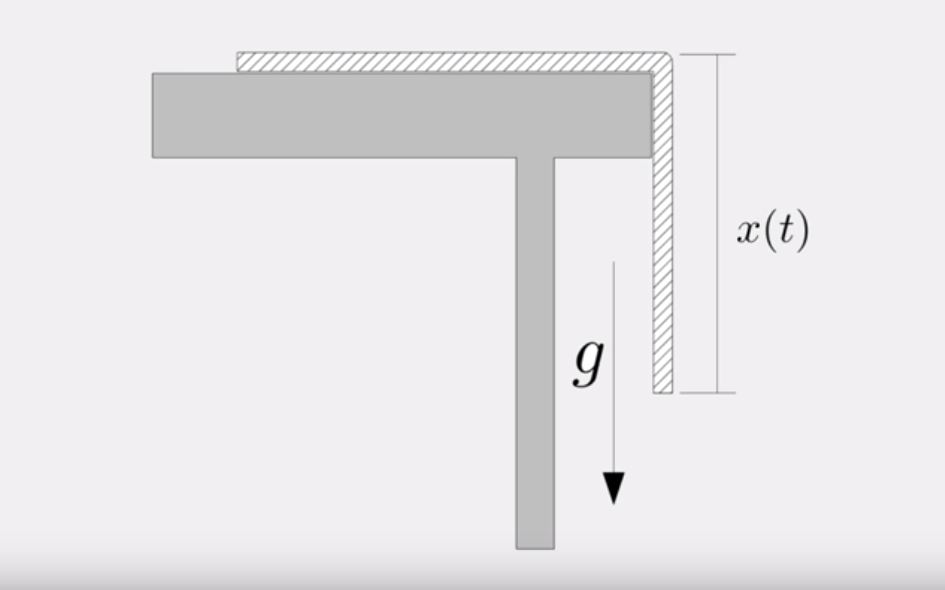
\includegraphics[width=8cm]{ropemass}
		\end{center}
		
	\end{q}
	
	\begin{q}
		\textbf{The Tautochrone} - the curve down which a particle will slide freely under gravity alone, reaching the bottom in time regardless of its starting point on the curve. \\
		A figure of the curve is shown on the side. The starting point is $ P(a,b) $ and the end point is the origin. \\ 
		\begin{center}
			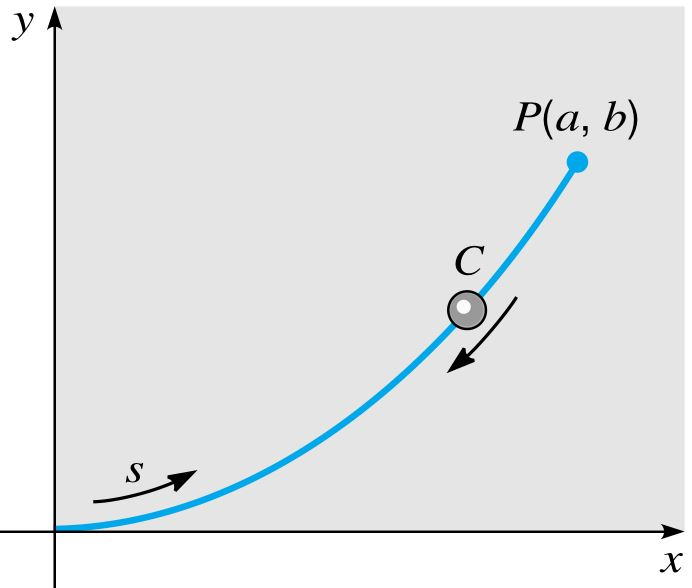
\includegraphics[width=8cm]{taut} 
		\end{center}
		\begin{enumerate}
			\item Given that the Arc length $ s $ is measured from the origin and $ f(y) $ gives the rate of change of $ s $ with respect to $ y $. 
			\[ f(y) = \dfrac{ds}{dy} = \left[1 + \left( \dfrac{dx}{dy} \right)^2 \right]^{1/2} \]
			\item Using conservation of energy the time $ T(b) $ required for a particle to slide from $ P $ to the origin is (Show this step!!)
			\[ T(b) = \dfrac{1}{\sqrt{2g}} \int_{0}^{b}\dfrac{f(y)}{\sqrt{b-y}} dy\]
			\item By the property of a Tautochrone the value of $ T(b) = T_0 $ is a constant for each $ b $. Taking the Laplace transform show that 
			\[ F(s) = \sqrt{\dfrac{2g}{\pi}} \dfrac{T_0}{\sqrt{s}} \] 
			\item Then show that 
			\[ f(y) = \dfrac{\sqrt{2g}}{\pi} \dfrac{T_0}{\sqrt{y}}\] 
			\item Using the previous answers show 
			\[ \dfrac{dx}{dy} = \sqrt{\dfrac{2 \alpha - y}{y}} \]
			where $ \alpha = gT_0^2/\pi^2 $ 
			\item Use the substitution $ y = 2 \alpha \sin ^2 (\theta / 2)$ and show 
			\[ x = \alpha (\theta + \sin \theta) \] \[ y = \alpha (1-\cos \theta)\] 
			Which is a parametric equation of a cycloid, the solution to the problem
		\end{enumerate}
	\end{q}
\end{multicols*}